%%%%%%%%%%%%%%%%%%%%%%%%%%%%%%%%%%%%%%%%%%%%%%%%%%%%%%%%%%%%%%%%%
% Contents: The home chapter
% $Id: grisbi-manuel-home.tex, v 0.4 2002/10/27 Daniel Cartron
% $Id: grisbi-manuel-home.tex, v 0.5.0 2004/06/01 Loic Breilloux
% $Id: grisbi-manuel-home.tex, v 0.6.0 2011/11/17 Jean-Luc Duflot
% some of its content was in menus chapter:
% $Id: grisbi-manuel-menus.tex, v 0.5.0 2004/06/01 Loic Breilloux
% $Id: grisbi-manuel-home.tex, v 0.8.9 2012/04/27 Jean-Luc Duflot
% $Id: grisbi-manuel-home.tex, v 1.0 2014/02/12 Jean-Luc Duflot
%%%%%%%%%%%%%%%%%%%%%%%%%%%%%%%%%%%%%%%%%%%%%%%%%%%%%%%%%%%%%%%%%

\chapter{Entrée dans Grisbi\label{entrance}}

\section{Sélection d'un fichier\label{select-file}}

\vspacepdf{5mm}			% vertical space = 5 mm

Au lancement de l'application, Grisbi affiche la page qui vous permet de démarrer de différentes manières.

\vspacepdf{5mm}			% espace : 5 mm

Vous pouvez afficher la fenêtre de Grisbi en \indexword{plein écran}\index{affichage!plein écran}\index{plein écran!affichage} par la touche de fonction \key{F11}, et revenir en arrière par la même touche.			% "!" separates the term from the subterm of the index entry

\vspacepdf{5mm}			% espace : 5 mm

%\ifIllustration
\begin{figure}[htbp]			% h=here, t=top, b=bottom, p=page of float to force the figure here, not in a next page.
	\begin{center}					% image centrée
		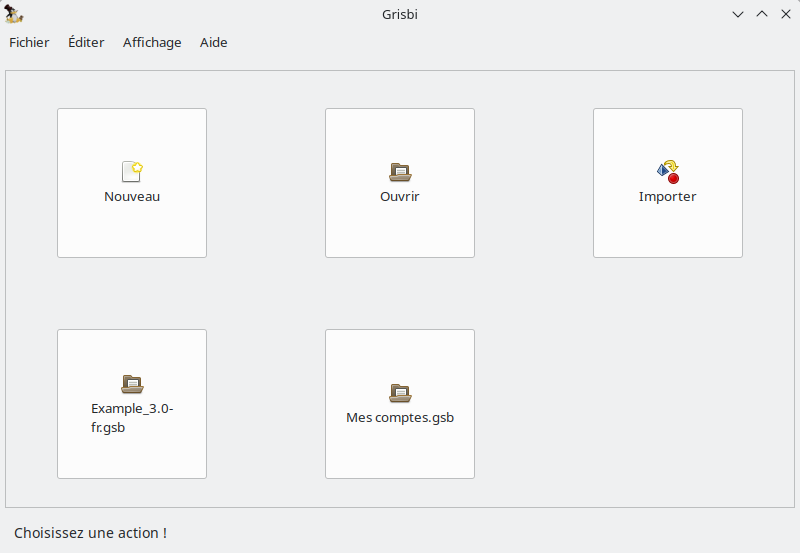
\includegraphics[width=0.95\textwidth]{image/screenshot/start_grisbi}		% width=95% as wide as the current text
	\end{center}
	\caption{Fenêtre de démarrage}			% sous-titre/subtitle
	\label{start_grisbi}					% figure's ref., use for link in text with \refimage{}
\end{figure}
%\fi

\vspacepdf{3mm}			% espace : 5 mm

En plus de la barre de menu, cette fenêtre affiche plusieurs pavés:

\begin{itemize}
	\item le pavé Nouveau, pour lancer l'assistant \frquote{Aide à la création d'un nouveau fichier de comptes};
	\item le pavé Ouvrir, pour afficher un gestionnaire de fichier avec lequel vous pourrez chercher un fichier de comptes existant dans votre ordinateur;
	\item le pavé Importer, pour lancer l'assistant \frquote{Importation des opérations par Grisbi};
	\item un ou plusieurs autres pavés, portant le nom de fichiers de comptes que Grisbi a déjà utilisés.
\end{itemize}


\textbf{Note}: les pavés portant les noms des fichiers de comptes que Grisbi a déjà utilisés ne sont présents que si ces fichiers existent; si vous voulez les enlever de cette page d'entrée, déplacez-les dans un autre répertoire, ou supprimez-les.

\vspacepdf{5mm}			% espace : 5 mm

En bas de page, un bandeau vous appelle à choisir une action en sélectionnant l'un de ces pavés.

\vspacepdf{5mm}			% espace : 5 mm

Si vous voulez juste découvrir le logiciel Grisbi pour avoir un aperçu de son aspect et de ses possibilités, vous pouvez à la place utiliser un fichier exemple comme celui présent sur le site de \lang{Sourceforge.net}\footnote{\urlSourceForgeDocumentation{}} dans le dossier \frquote{\textsf{examples}}.		% (voir la section \vref{new-example}).

\vspacepdf{5mm}			% espace : 5 mm

\textbf{Note}: en cliquant simplement sur le fichier exemple téléchargé, Grisbi s'exécutera en affichant directement la fenêtre d'accueil\refimage{home_3.0} sans passer par la fenêtre de démarrage.


\section{Accueil\label{home}}

\vspacepdf{5mm}

En ouvrant un fichier de comptes, Grisbi affiche sa page d'accueil\refimage{home_3.0}.
C'est la page de démarrage du programme; on peut y accéder à tout moment en cliquant sur l'onglet \menu{Comptes}. 

\vspacepdf{3mm}

\begin{figure}[htbp]			% h=here, t=top, b=bottom, p=page of float to force the figure here, not in a next page.
\begin{center}
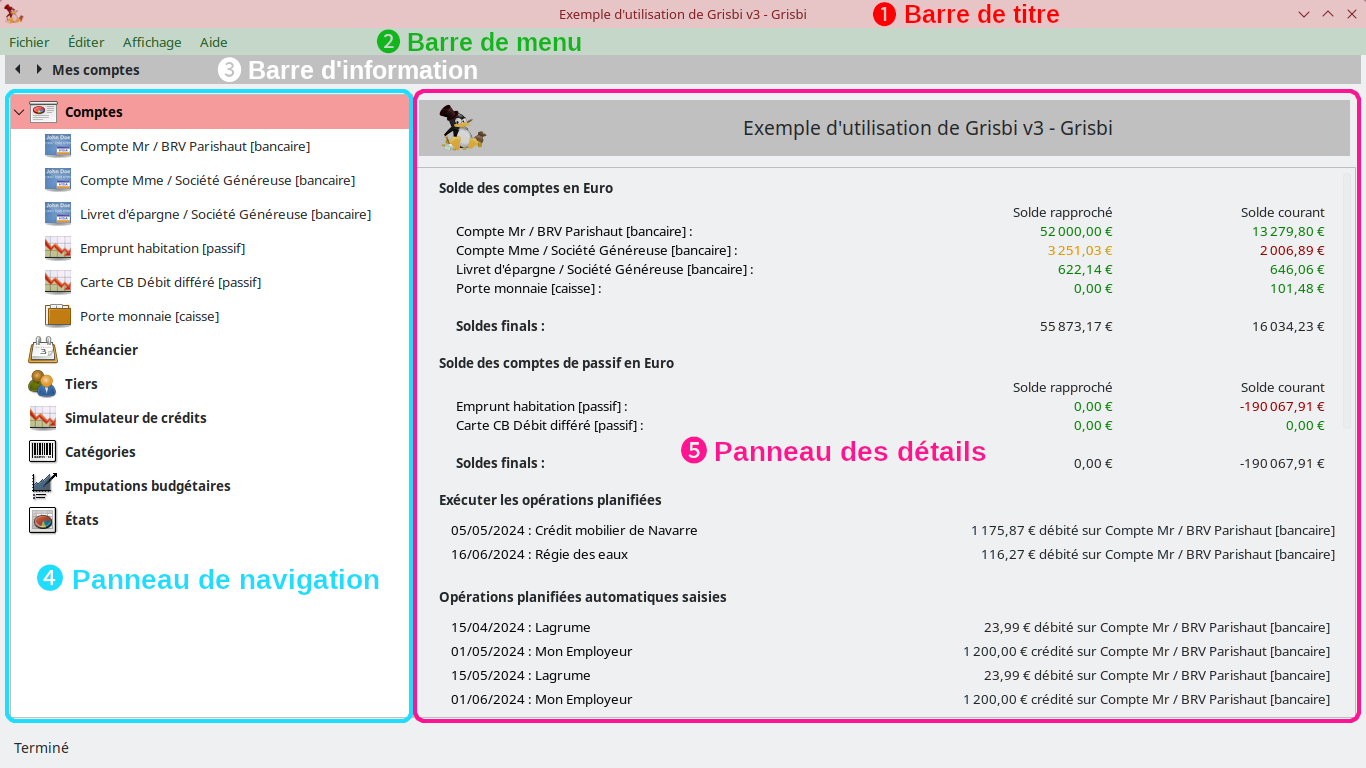
\includegraphics[width=1\textwidth]{image/screenshot/home_3.0.png}
\end{center}
\caption{Page d'accueil}		% sous-titre/subtitle
\label{home_3.0}
\end{figure}

\vspacepdf{3mm}

Grisbi affiche toutes ses pages de la même manière: comme n'importe quel logiciel, il affiche:% une barre de titre, une barre de menus qui donne accès à la plupart des fonctionnalités importantes de Grisbi, et aussi trois zones:

\begin{itemize}%[\large \textcircled{\small 2}]
	\item[\large\textcircled{\small 1}] une barre de titre;
	\item[\large\textcircled{\small 2}] une barre de menus qui donne accès à la plupart des fonctionnalités importantes de Grisbi;
\end{itemize}
et aussi trois zones qui sont spécifiques à Grisbi:
\begin{itemize}%[3,4,5]
	\item[\large\textcircled{\small 3}] la barre d'information, sous la barre de menus;
	\item[\large\textcircled{\small 4}] le panneau de navigation;
	\item[\large\textcircled{\small 5}] le panneau des détails
\end{itemize}

%Les zones 3, 4 et 5 sont spécifiques à Grisbi%, sont encadrées de couleurs dans la figure pour bien les identifier\refimage{home}.


\section{Barre d'information\label{home-synthesis}}


La barre d'information affiche le nom de l'onglet courant affiché, et peut afficher, complètement à droite, certains soldes en rapport avec ce qui est sélectionné dans le pavé des détails.

% espace pour changement de thème
\vspacepdf{5mm}
Elle permet, en cliquant successivement sur l'un des deux petits triangles à sa gauche, de sélectionner l'un des onglets affichés dans le panneau de navigation: \menu{Comptes}, \menu{Échéancier}, \menu{Tiers}, \menu{Simulateur de crédits}, \menu{Catégories}, \menu{Imputations budgétaires} et \menu{États}, et aussi l'un des sous-onglets des onglets \menu{Comptes} et \menu{États} s'ils sont déroulés dans le panneau de navigation.

\vspacepdf{5mm}
% Pas de commande au clavier pour cette fonction
\textbf{Note}: ces triangles peuvent être remplacés, en fonction du thème de l'environnement de bureau ou du gestionnaire de fenêtres que vous utilisez, par d'autres caractères tels que +, -, >, <, etc.

% espace pour changement de thème
\vspacepdf{3mm}
Le contenu de la sélection s'affiche dans le pavé des détails.

% espace pour changement de thème
\vspacepdf{3mm}
Ces fonctionnalités peuvent être utilisées à la place de celles du panneau de navigation lorsque sa largeur est réduite à zéro et que l'on n'y a pas accès directement.


\section{Panneau de navigation\label{home-accounting}}


Le panneau de navigation affiche en caractères gras la liste des onglets: \menu{Comptes}, \menu{Échéancier}, \menu{Tiers}, \menu{Simulateur de crédits}, \menu{Catégories}, \menu{Imputations budgétaires} et \menu{États}. En cliquant sur le petit triangle noir à gauche des onglets \menu{Comptes} ou \menu{États}, on peut dérouler ou enrouler la liste de leurs sous-onglets. Vous pouvez changer l'ordre des onglets et des sous-onglets en cliquant sur l'un d'eux et en le déplaçant plus haut ou plus bas dans la liste.

\vspacepdf{3mm}

\textbf{Note}: ces triangles peuvent être remplacés, en fonction du thème de l'environnement de bureau ou du gestionnaire de fenêtres que vous utilisez, par d'autres caractères tels que +, -, >, <, etc.

% espace pour changement de thème
\vspacepdf{5mm}
Vous pouvez sélectionner un de ces onglets ou sous-onglets en cliquant sur son nom. Vous pouvez aussi déplacer la sélection dans cette liste d'onglets et de sous-onglets avec les touches du clavier \key{Flèche Haut}, \key{Flèche Bas}, \key{Pg. Préc} ou \key{Pg. Suiv}, ou avec la molette de la souris. 

% espace pour changement de thème
\vspacepdf{5mm}
Le contenu de la sélection s'affiche dans le pavé des détails. 

% espace pour changement de thème
\vspacepdf{5mm}
On peut réduire ou agrandir la largeur du panneau de navigation en cliquant sur la fine barre verticale entre ce panneau et le pavé des détails, et en la déplaçant. Si la largeur du panneau a été réduite à zéro, ou agrandie au maximum de la largeur de la fenêtre de Grisbi, il faut retrouver cette barre, respectivement complètement à gauche ou à droite de la fenêtre, et la faire glisser à la place désirée. 

% espace pour changement de thème
\vspacepdf{5mm}
Des \indexword{menus contextuels}\index{menu contextuel}, accessibles par un clic-droit de souris, sont disponibles sur les éléments de ce panneau et proposent les fonctions suivantes:

\begin{itemize}
	\item sur \menu{Comptes}:
		\begin{itemize}
			\item \menu{Nouveau compte};
			\item sur un compte quelconque: 
				\begin{itemize}
					\item \menu{Nouveau compte},
					\item \menu{Supprimer ce compte};
				\end{itemize}
		\end{itemize}
	\item sur \menu{Tiers}:
		\begin{itemize}
			\item \menu{Nouveau tiers},
			\item \menu{Supprimer le tiers sélectionné},
			\item \menu{Éditer le tiers sélectionné},
			\item \menu{Gérer les tiers},
			\item \menu{Supprimer les tiers inutilisés};
		\end{itemize}
	\item sur \menu{Catégories}: 
		\begin{itemize}
			\item \menu{Nouvelle catégorie},
			\item \menu{Supprimer la catégorie sélectionnée},
			\item \menu{Editer la catégorie sélectionnée},
			\item \menu{Importer un fichier de catégories (.csgb)},
			\item \menu{Exporter la liste des catégories (.csgb)};
		\end{itemize}
	\item sur \menu{Imputations budgétaires}:
		\begin{itemize}
			\item \menu{Nouvelle imputation budgétaire},
			\item \menu{Supprimer l'imputation sélectionnée},
			\item \menu{Editer l'imputation sélectionnée},
			\item \menu{Importer un fichier d'imputations budgétaires (.isgb)},
			\item \menu{Exporter la liste des imputations budgétaires (.isgb)};
		\end{itemize}
	\item sur \menu{État}:
		\begin{itemize}
			\item \menu{Nouvel état};
			\item sur un état quelconque: 
				\begin{itemize}
					\item \menu{Nouvel état},
					\item \menu{Supprimer cet état}.
				\end{itemize}
		\end{itemize}
\end{itemize}

% saut de page pour titre solidaire
%\newpage


\section{Panneau des détails\label{home-details}}


Le pavé des détails affiche tous les détails sur les onglets ou sous-onglets sélectionnés par la barre d'information ou le panneau de navigation. C'est la zone de travail principale de Grisbi.

On peut réduire ou agrandir sa largeur en cliquant sur la fine barre verticale entre ce panneau et le panneau de navigation, et en la déplaçant. Si la largeur du panneau a été réduite à zéro ou agrandie au maximum de la largeur de la fenêtre de Grisbi, il faut retrouver cette barre, respectivement complètement à droite ou à gauche de la fenêtre, et la faire glisser à la place désirée. 
 
%%TODO%: LA SUITE
 
\subsection{Affichage de la page d'accueil\label{home-details-homepage}}

Pour afficher la page d'accueil, sélectionnez l'onglet \menu{Comptes}; le panneau des détails affiche, de haut en bas:

\begin{itemize}
	 \item dans un pavé sur fond gris, l'icône \menu{Grisbi} à gauche, et à droite un \indexword{titre}\index{affichage!titre}\index{titre!page d'accueil} qui permet d'identifier sur quelle comptabilité vous travaillez actuellement, sous la forme \frquote{libellé - Grisbi}; vous pouvez définir ce libellé, parmi trois possibilités, dans le menu \menu{Édition - Préférences} (voir le paragraphe \vref{setup-display-addresses-titles}, \menu{Titres}):
		\begin{itemize}
			 \item l'\menu{Entité comptable}: c'est le nom du domaine de comptabilité sur lequel vous travaillez, par exemple \frquote{Ma comptabilité} ou \frquote{Association}, et que vous avez saisi à la création du fichier de comptes; vous pouvez le modifier ici dans le champ \menu{Nom de l'entité comptable}; cela peut être utile si vous gérez plusieurs \indexword{entités comptables}\index{entité comptable}, 
			 \item le \menu{Titulaire du compte}: c'est le nom du titulaire (ou du propriétaire) du dernier compte consulté; si le titulaire n'est pas renseigné dans les propriétés du compte, Grisbi affiche le nom de ce compte,
			 \item le \menu{Nom du fichier de comptes}: c'est le nom du fichier dans le répertoire courant, sous la forme \file{nom\_de\_\_votre\_fichier.gsb}, et c'est le choix par défaut;
		\end{itemize}
	 \item pour chaque devise séparément, pour tous les comptes et \indexword{groupes de comptes}\index{groupe de comptes}, sous les libellés \menu{Solde rapproché} et \menu{Solde courant}:
		\begin{itemize}
			 \item le solde des comptes bancaires et comptes de caisse, le solde partiel des groupes de comptes et leur solde final,
% saut de ligne pour indentation correcte de la note dans la liste

			 \textbf{Note}: vous pouvez ajuster l'ordre d'affichage des soldes partiels des groupes de comptes (voir le paragraphe \vref{setup-general-home-partBalance}, \menu{Soldes partiels de la liste des comptes}).			 
			 \item le solde des comptes de passif et leur solde final,
			 \item le solde des comptes d'actif et leur solde final;
		\end{itemize}
	\item les \indexword{alertes des opérations planifiées}\index{alerte!opération planifiée} à échéance ou clôturées, avec leurs date, libellé et montant, selon les choix faits dans le menu \menu{Édition - Préférences} (voir la section \vref{setup-general-planned}, \menu{Échéancier});
	\item la liste des comptes dont le solde est passé sous le \menu{Solde minimal autorisé};
	\item la liste des comptes dont le solde est passé sous le \menu{Solde minimal voulu}.
\end{itemize}

% espace avant Attention ou Note: 5 mm
\vspacepdf{5mm}

\textbf{Note}: pour les définitions du \menu{Solde minimal autorisé} et du \menu{Solde minimal voulu}, voir la section \vref{accounts-properties}, \menu{Propriétés d'un compte}.

% espace pour changement de thème
\vspacepdf{5mm}
Les libellés des comptes s'affichent en \textcolor{black}{noir}; au passage du pointeur de la souris sur la ligne de l'un d'eux, cette couleur passe au \textcolor{gray}{gris}.
Un solde supérieur au \menu{Solde minimal voulu} s'affiche en \textcolor{teal}{vert foncé}; au passage du pointeur sur sa ligne, cette couleur passe au \textcolor{lime}{vert clair}.
Un solde inférieur au \menu{Solde minimal voulu} et supérieur au \menu{Solde minimal autorisé} s'affiche en \textcolor{orange}{orange}; au passage du pointeur sur sa ligne, cette couleur passe à l'\textcolor{orange}{orange clair}.
Un solde inférieur au \menu{Solde minimal autorisé} s'affiche en \textcolor{red}{rouge}; au passage du pointeur sur sa ligne, cette couleur passe au \textcolor{red}{rouge clair}.

Au passage du pointeur de la souris sur la ligne d'un compte, tout changement de couleur indique que si l'on clique (droit ou gauche) avec la souris, ce compte s'affiche, comme s'il avait été sélectionné avec la barre d'information ou le panneau de navigation; il affiche alors la page qui contient la ligne d'opération affichant ce solde.

Un solde partiel, qui correspond à un groupe de comptes, s'affiche en \textcolor{black}{noir}. S'il est négatif, il peut s'afficher en \textcolor{red}{rouge foncé}, mais seulement si cela a été configuré ainsi (voir le paragraphe \vref{setup-general-home-partBalance}, \menu{Soldes partiels de la liste des comptes}). Une ligne de solde partiel ne change pas de couleur au passage du pointeur de la souris dessus, car on ne peut pas afficher les opérations d'un groupe de comptes.

% espace pour changement de thème
\vspacepdf{5mm}
Vous pouvez configurer certains aspects de l'affichage de cette page d'accueil dans le menu \menu{Édition - Préférences} ou dans l'onglet \menu{Propriétés} de chaque compte:
\begin{itemize}
	 \item \menu{\indexword{Polices}\index{polices}, \indexword{logo}\index{logo} et \indexword{couleurs}\index{couleurs}}: section \vref{setup-display-logo};
	 \item \menu{Titres}: section \vref{setup-display-addresses-titles};
	 \item \menu{Calcul des soldes}: paragraphe \vref{setup-general-home-balance};
	 \item \menu{Soldes partiels de la liste des comptes}: paragraphe \vref{setup-general-home-partBalance};
	 \item \menu{Alertes de l'échéancier}: section \vref{setup-general-planned};
	 \item comptes sous le \menu{\indexword{Solde minimal autorisé}}\index{solde!minimal autorisé}: section \vref{accounts-properties};
	 \item comptes sous le \menu{\indexword{Solde minimal voulu}}\index{solde!minimal voulu}: section \vref{accounts-properties}.
\end{itemize}

En particulier, si vous trouvez une erreur d’orthographe dans cette page, vous pourrez la corriger: voir le paragraphe \vref{setup-general-home-final}, \menu{Pluriel de final}!

%\ifIllustration
% saut de page pour paragraphe solidaire
%\newpage
%\fi

\section{Barre de menus\label{home-menus}}


Comme dans de nombreuses applications graphiques, la plupart des fonctionnalités importantes de Grisbi sont accessibles au moyen des menus de la \indexword{barre de menus}\index{barre de menus}. Nous détaillons ici leurs fonctionnalités.


\subsection{Menu \menu{Fichier}\label{home-menus-file}}

Ce menu comprend les fonctions suivantes:

\begin{itemize}
	\item \menu{Nouveau fichier de comptes}: crée un nouveau fichier de comptes; le fichier courant est donc fermé et un nouveau fichier vide est créé avec un compte vide (raccourci-clavier \key{Ctrl}\key{N}), voir la section \vref{start-newfile}; à ne pas confondre avec la création d'un nouveau compte;
	\item \menu{Ouvrir}: ouvre un fichier de comptes (raccourci-clavier \key{Ctrl}\key{O});
	\item \menu{Derniers fichiers}: affiche la liste des n derniers fichiers ouverts avec Grisbi (seulement s'il y en a eu plusieurs); ce nombre est configurable dans le menu \menu{Edition - Préférences}, voir la section \vref{setup-general-files-manage}, \menu{Gestion des fichiers de compte};
	\item \menu{Enregistrer} enregistre le fichier de comptes en cours (raccourci-clavier \key{Ctrl}\key{S});
	\item \menu{Enregistrer sous}: ouvre un gestionnaire de fichiers pour enregistrer le fichier de comptes en cours avec le nom et à l'emplacement de 	votre choix; Grisbi vous propose par défaut le répertoire courant, le nom du fichier de comptes en cours, avec l'extension \file{.gsb};
	\item \menu{Importer un fichier}: démarre l'assistant d'importation de fichiers d'un autre logiciel; voir la section \vref{move-import-importinit};
	\item \menu{Exporter vers un fichier QIF/CSV}: démarre l'assistant d'exportation de fichiers de compte; voir la section \vref{move-export};	
	\item \menu{Créer une archive}: démarre l'assistant de création d'archive; voir la section \vref{datamanagement-history-new};	
	\item \menu{Exporter une archive vers un fichier GSB/QIF/CSV}: démarre l'assistant d'exportation d'archive; voir la section \vref{datamanagement-history-export};
	\item \menu{Déboguer le fichier de compte}: démarre l'assistant de 	débogage de ce fichier, qui va vous aider à chercher des incohérences dans votre fichier de comptes; voir la section \vref{maintenance-file-debug};
	\item \menu{Rendre anonyme le fichier de comptes}: démarre l'assistant qui produit une copie anonymée de votre fichier de comptes; ce fichier pourra être joint à un rapport de bogue; voir la section \vref{maintenance-file-anonymous};	
	\item \menu{Rendre anonyme le fichier QIF}: démarre l'assistant qui produit une copie anonymée de ce fichier; ce fichier pourra être joint à un rapport de bogue; voir la section \vref{maintenance-QIF-anonymous};	
	\item \menu{Mode de débogage}: met Grisbi en mode de débogage, qui crée un fichier-journal des évènements; voir la section \vref{maintenance-debug-mode}; 	
	\item \menu{Fermer}: ferme le fichier de comptes en cours; Grisbi vous propose de l'enregistrer si ce n'est déjà fait (raccourci-clavier \key{Ctrl}\key{W});
	\item \menu{Quitter}: ferme Grisbi; Grisbi vous propose auparavant d'enregistrer le fichier de comptes, si ce n'est pas déjà fait (raccourci-clavier \key{Ctrl}\key{Q}).
\end{itemize}


\subsection{Menu \menu{Édition}\label{home-menus-edit}}

Ce menu comprend les fonctions suivantes:

\begin{itemize}
	\item \menu{Editer l'opération}: voir la section \vref{transactions-modify}, \menu{Modification d'une opération};
	\item \menu{Nouvelle opération}: voir la section \vref{transactions-new}, \menu{Saisie d'une nouvelle opération};
	\item \menu{Supprimer une opération}: voir la section \vref{transactions-delete}, \menu{Suppression d'une opération};
	\item \menu{Utiliser l'opération sélectionnée comme modèle}: voir la section \vref{transactions-model}, \menu{Opération sélectionnée comme modèle};
	\item \menu{Cloner l'opération}: voir la section \vref{transactions-duplicate}, \menu{Clonage d'une opération};
	\item \menu{Convertir en opération planifiée}: voir la section \vref{transactions-schedule}, \menu{Conversion d'une opération en opération planifiée};
	\item \menu{Déplacer l'opération vers un autre compte}: voir la section \vref{transactions-move}, \menu{Déplacement d'une opération vers un autre compte};
	\item \menu{Nouveau compte}: voir la section \vref{accounts-new}, \menu{Création d'un nouveau compte};
	\item \menu{Supprimer le compte courant}: voir la section \vref{accounts-delete}, \menu{Suppression d'un compte};
	\item \menu{Préférences}: permet de configurer Grisbi; voir le chapitre \vref{setup}, \menu{Configuration de Grisbi}.
\end{itemize}


\subsection{Menu \menu{Affichage}\label{home-menus-display}}

Ce menu comprend les fonctions suivantes; 

\begin{itemize}
	 \item \menu{Montrer le formulaire de saisie d'opérations}; 
	 \item \menu{Montrer les opérations rapprochées} (raccourci-clavier \key{Alt}\key{R});
	 \item \menu{Montrer les lignes d'archives} (raccourci-clavier \key{Altl}\key{L});
	 \item \menu{Montrer les \indexword{comptes clos}}\index{compte!clos};
	 \item \menu{Montrer une ligne par opération};
	 \item \menu{Montrer deux lignes par opération};
	 \item \menu{Montrer trois lignes par opération};
	 \item \menu{Montrer quatre lignes par opération};
	 \item \menu{Réinitialiser la largeur des colonnes}; permet de remettre les colonnes des listes d'opérations à leur largeur d'origine.
\end{itemize}


\subsection{Menu \menu{Aide}\label{home-menus-help}}

La plupart des choix de ce menu donnent accès à des sites Web. Pour que ces accès fonctionnent, il faut avoir indiqué à Grisbi le logiciel de navigation (ou navigateur) que vous souhaitez utiliser, dans le menu \menu{Édition - Préférences} (voir la section \vref{setup-general-programs}, \menu{Programmes}). Le menu \menu{Aide} comprend les choix suivants;

\begin{itemize}
	\item \menu{Manuel}; ouvre votre navigateur à la page \frquote{Manuel de l'Utilisateur de Grisbi} (raccourci-clavier \key{Ctrl}\key{H});
	\item \menu{Démarrage rapide}; ouvre votre navigateur à la page \frquote{Démarrage Rapide de Grisbi};
	\item \menu{Traduction}; ouvre votre navigateur à la page \frquote{Traduire Grisbi}, pour vous inviter à nous aider à l'élargissement de 	l'internationalisation de Grisbi;
	\item \menu{À propos de Grisbi}; affiche la boîte d'information sur l'application; vous y trouverez des détails sur la version, le lien vers le site de Grisbi, les remerciements (contributeurs au projet) et la licence d'utilisation;
	\item \menu{Site Web de Grisbi}; ouvre votre navigateur à la page du site de \lang{Grisbi}\footnote{\urlGrisbi{}};
	\item \menu{Signaler une anomalie}; ouvre votre navigateur à la page du \lang{traqueur de bogues de Grisbi}\footnote{\urlBugTracker{}} pour vous permettre de signaler un bogue que vous auriez découvert. Vous pouvez également suivre sur cette page l'évolution des corrections apportées aux bogues signalés;
	\item \menu{Astuce du jour}; ouvre une boîte de dialogue qui affiche une astuce d'utilisation, différente à chaque démarrage de Grisbi; vous pouvez y 	afficher successivement toutes les astuces, et choisir ou non l'affichage de 	l'astuce du jour au démarrage de Grisbi. Pour supprimer ou réactiver l'astuce du 	jour, voir le paragraphe \vref{setup-display-messages-trick}, \menu{Astuce du jour}.
\end{itemize}


\section{Raccourcis-clavier\label{home-shortcuts}}


Les raccourcis-clavier facilitent la saisie des données et la navigation dans les fenêtres de Grisbi, en évitant le recours systématique au déplacement et au clic de la souris. En utilisant ceux correspondant aux manipulations les plus courantes pour vous, vous améliorez votre \indexword{ergonomie}\index{ergonomie} en limitant les mouvements importants de vos bras.
 
Grisbi dispose d'un certain nombre de raccourcis-clavier, présentés ici selon différents thèmes (voir aussi la section \vref{introduction-manual-conventions}, \menu{Conventions typographiques du présent manuel}).


\subsection{Application et fichiers}

\begin{itemize}
	\item Nouveau fichier de comptes; \key{Ctrl}\key{N}
	\item Ouvrir un fichier de comptes: \key{Ctrl}\key{O}
	\item Enregistrer le fichier de comptes: \key{Ctrl}\key{S}
	\item Fermer le fichier de comptes: \key{Ctrl}\key{W}
	\item Fermer Grisbi: \key{Ctrl}\key{Q}
\end{itemize}


\subsection{Panneau de navigation}

\begin{itemize}
	\item Sélectionner un onglet ou un compte: \key{Flèche Haut}, \key{Flèche Bas}, \key{Page Haut} ou \key{Page Bas}
\end{itemize}


\subsection{Liste des opérations et des opérations planifiées}

\begin{itemize}
	\item Sélectionner une opération: \key{Entrée}
	\item Déplacer la sélection: \key{Flèche Haut} ou \key{Flèche Bas}
	\item Nouvelle opération: \key{Entrée} sur ligne vide, ou \key{Ctrl}\key{T}
	\item Modifier une opération: \key{Entrée}
	\item Supprimer une opération: \key{Suppr};
	\item Pointer ou dépointer une opération: \key{Ctrl}\key{P}
	\item Rapprocher ou dérapprocher une opération: \key{Ctrl}\key{R}
	\item Montrer ou masquer les opérations rapprochées: \key{Alt}\key{R}
	\item Montrer ou masquer les lignes d'archives: \key{Altl}\key{L}
\end{itemize}


\subsection{Formulaire de saisie }

\begin{itemize}
	\item La touche \key{Entrée} est configurable: elle permet soit de se déplacer dans le formulaire de saisie, soit de valider l'entrée
	\item Se déplacer au champ suivant: \key{Tabulation} (selon votre choix de configuration)
	\item Annuler la saisie en cours: \key{Échap}
	\item Accepter l'auto-complètement: \key{Tabulation} ou \key{Entrée} (selon votre choix de configuration)
	\item Symbole de l'euro: \key{AltGr}\key{e}
\end{itemize}


\subsection{Listes déroulantes}

\begin{itemize}
	 \item Ouvrir une liste: \key{Page Bas} ou \key{Flèche bas}
	 \item Se déplacer dans la liste: \key{Flèche haut}, \key{Flèche bas}, \key{Page Haut} ou \key{Page Bas}
	 \item Valider un choix à l'intérieur d'une liste: \key{Entrée}
	 \item Devises, exercices et modes de règlement:
		\begin{itemize}
			\item ouvrir la liste: \key{Espace}; 
			\item se déplacer dans la liste: \key{Flèche Haut} ou \key{Flèche Bas};
			\item valider l'item de la liste: \key{Espace}.
		\end{itemize}
\end{itemize}


\subsection{Dates saisies au calendrier}

\begin{itemize}
	\item Ouvre un calendrier (sur le champ de date): \key{Ctrl}\key{Entrée}
	\item Ferme le calendrier sans modifier la date: \key{Échap}
	\item Valide la date sélectionnée: \key{Entrée}
	\item Jour suivant ou précédent: \key{+} ou \key{-}, \key{Flèche Droite} ou \key{Flèche Gauche}
	\item Semaine précédente ou suivante: \key{Flèche Haut} ou \key{Flèche Bas}
	\item Mois précédent ou suivant: \key{Page Haut} ou \key{Page Bas}
	\item Premier jour ou dernier jour du mois: \key{Début} ou \key{Fin}
\end{itemize}


\subsection{Dates saisies au clavier}

\begin{itemize}
	\item Jour suivant ou précédent: \key{+} ou \key{-}
	\item Semaine précédente ou suivante: \key{Majuscule} \key{+} ou \key{Majuscule} \key{-}
	\item Mois précédent ou suivant: \key{Page Haut} ou \key{Page Bas}
	\item Année précédente ou suivante: \key{Majuscule} \key{Page Haut} ou \key{Majuscule} \key{Page Bas}
	\item Valide la date sélectionnée \key{Entrée}
\end{itemize}


\subsection{Tiers, catégories, imputations budgétaires, simulateur de crédits, données historiques et prévisions}

\begin{itemize}
	\item Déplacer la sélection: \key{Flèche Haut}, \key{Flèche Bas}, \key{Page Haut} ou \key{Page Bas}
%Ces raccourcis ne fonctionnent plus:
%	\item afficher les sous-catégories ou sous-imputations budgétaires (sur une catégorie ou une imputation budgétaire): \key{Espace};
%	\item afficher les opérations des sous-catégories ou sous-imputations budgétaires (sur une sous-catégorie ou une sous-imputation budgétaire): \key{Espace}.
\end{itemize}


\subsection{États et Configuration}

\begin{itemize}
	\item Sélectionner un autre onglet: \key{Flèche Haut}, \key{Flèche Bas}, \key{Page Haut}, \key{Page Bas}
	\item Naviguer entre le panneau des onglets et les différentes options du panneau des réglages: \key{Tabulation}, \key{Flèche Haut}, \key{Flèche Bas}, \key{Flèche Gauche} et \key{Flèche Droit}
\end{itemize}

\subsection{Aide}

\begin{itemize}
	\item Ouvre votre navigateur à la page du Manuel de l'Utilisateur de Grisbi \key{Ctrl}\key{H}
\end{itemize}













